%% Introduction
%%=========================================

\chapter{Introduction}
The Oxford English Dictionary defines ``digitization" as the action or process of digitizing. Digitizing means the conversation of analogue data into digital form\cite{misc-oed-digitization}. As the world grows more and more digital, the need to digitize increases proportioned. In 2009, the National Library of Norway launched Bokhylla.no (The bookshelf). Bokhylla.no is a project to provide online access to literature published in Norwegian. The service will contain about 250 000 books when it is completed in 2017\cite{misc-nb-digial-library}. While simply scanning the books will suffice to make the literature available online, other technologies are needed to actually index the content.

While a scanner identifies the ink on the paper, it does not know, or care, which characters or symbols the ink is representing. In order to make sense of the scanned content, we use use optical character recognition, or OCR for short. OCR is the task of identifying printed characters and symbols using computer software. We can use OCR to index the entire content of the book, making it searchable. Indexed content can also be used to make the book accessible to blind and visually impaired users via text-to-speech technologies.

Countless research documents and theses are written in the field of optical character recognition. This task is critical in the digitization process.

\section{Context}
TODO

\section{Personal motivation}
TODO

\section{Goals}
The goal is to make OCR possible in a very limited search space. Several papers are already written on this field. While many of these papers focus on ``damaged" characters, or characters that are specially hard to classify, our goal is to use the ``signature" of a character to classify it.

By ``signature", we mean that we take characters and only use a horizontal line with a low height to classify it. In \ref{fig:thesis-signature} we have the word ``THESIS". The original characters have a height of 50 pixels, but to do our classification, we only use one pixel of the total height of the characters. The line that defines the signature for this word is highlighted in the figure for illustration purposes.

\begin{figure}[h]
    \centering
    
\includegraphics[width=0.7\textwidth]{fig/chapter1/signature.png}
    \caption{Illustration of a word with a signature with a height of one pixel}
    \label{fig:thesis-signature}
\end{figure}

The illustration in \ref{fig:thesis-signature} uses the sans-serif font Arial\cite{misc-arial-font}. As a \gls{sans-serif} font, the letters are clean, with no \gls{serif}s present. A few things are worth pointing out from the illustration to emphasise potential challenges with classifying via signatures.

\begin{itemize}
    \item The stroke from the T and the I are the same width, which makes them indistinguishable from each other.
    \item Because Arial is not monospaced, the spacing between each letter vary, depending on the letter before and their individual width.
\end{itemize}

\subsection{Example of use}
Markus ``Notch" Persson is a Swedish video game programmer and designer. He is most famous for crating the highly praised game Minecraft. During development of the game, Persson was a inveterate user of Twitter, and used to hint or tease upcoming features of the game. On June 12th 2011, Persson Tweeted the following Tweet:

\begin{figure}[h]
    \centering
    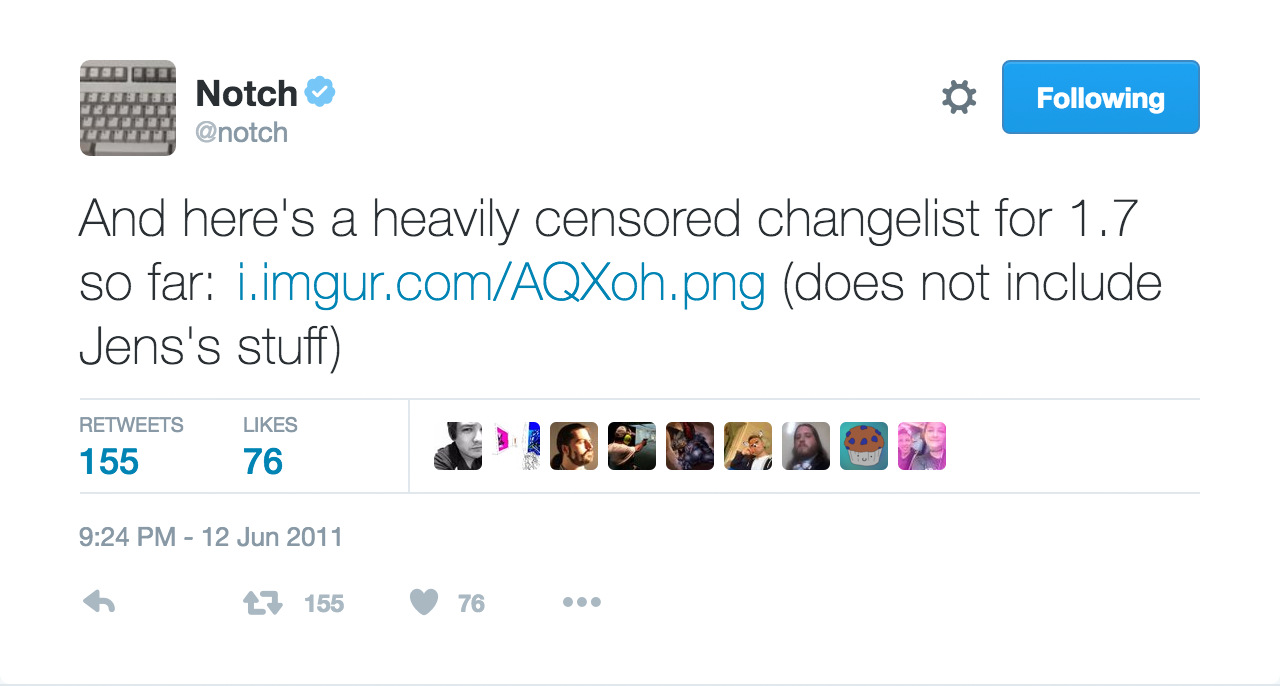
\includegraphics[width=0.7\textwidth]{fig/chapter1/notch_tweet.png}
    \caption{Print screen of Tweet from notch\protect\footnotemark}
\end{figure}
\footnotetext{Tweet and image used with the consent of Markus Persson. \href{https://twitter.com/notch/status/790531003169341440}{
    \nolinkurl{https://twitter.com/notch/}\\\nolinkurl{status/790531003169341440}}
}

The image he is referring to looks like this:

\begin{figure}[h]
    \centering
    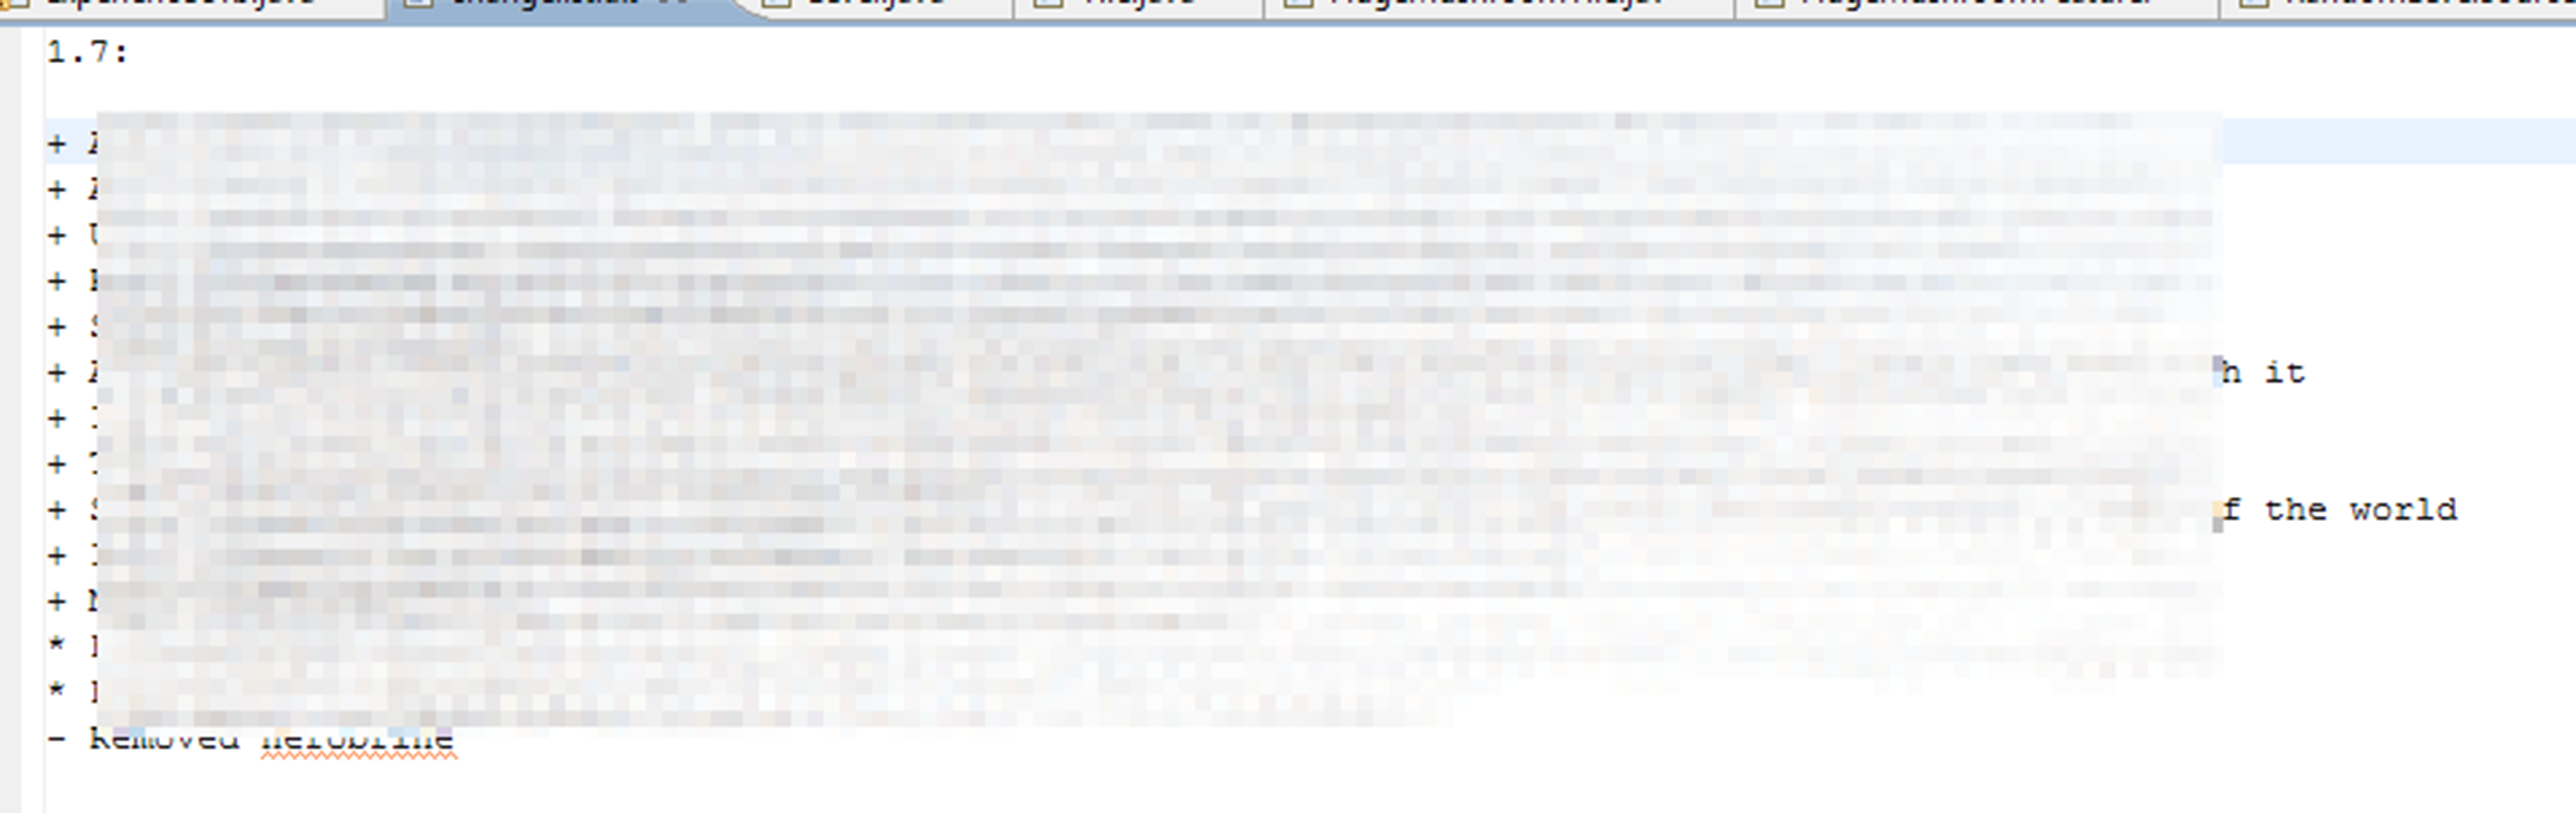
\includegraphics[width=0.7\textwidth]{fig/chapter1/notch_eclipse.png}
    \caption{Blurred image of Minecraft 1.7 changelog from @notch's Tweet}
\end{figure}

The image looks like it is taken inside a text editor or \gls{IDE}. There is a file currently opened, with several other files, or tabs, partially visible at the top of the image. The file that is currently opened seems to be a changelog for the upcoming 1.7 version of Minecraft, with the new major version written on the first line, followed by a list of changed. The content is mostly burred out, showing only parts of the first letter on each line and the content of some longer lines. The image is also cropped so that the file names for the files that are currently opened in the project is not displayed.

\section{Structure and approach}
TODO